\defbeamertemplate*{title page}{customized}[1][] {
%
%	\begin{tikzpicture}[remember picture,overlay]\node[at=(current page.center), opacity=0.8] {
%		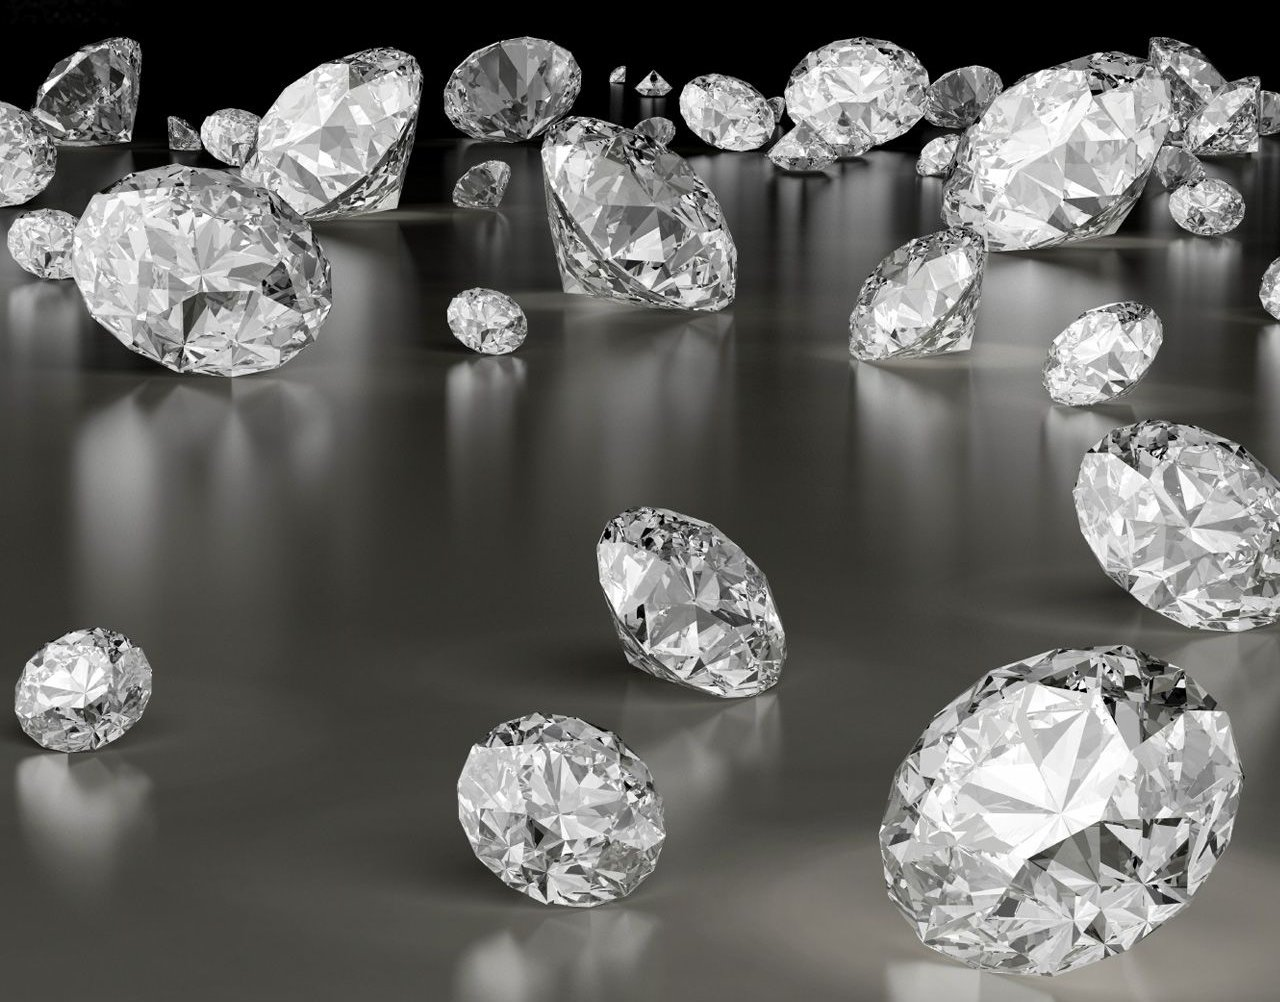
\includegraphics[width=1.14\paperwidth]{figures/main/bkg}};
%	\end{tikzpicture}
%
%	\begin{tcolorbox}[beamer, no shadow, opacityback=.6, opacityframe=.6, width=1.05\textwidth, grow to left by=5mm, left=1cm, top=5mm, bottom=5mm, interior style={top color=blue!20!green!50!white,bottom color=blue!20!yellow!50!white}]
	\begin{tcolorbox}[beamer, no shadow, opacityback=.6, opacityframe=.6, width=\paperwidth, grow to left by=5mm, left=1cm, top=5mm, bottom=5mm, interior style={top color=colone,bottom color=coltwo}]
		\begin{minipage}{.33\textwidth}\centering
			% PHOTO
			\roundphoto{\inserttitlegraphic}{3}
			% NAME
			\begin{tcolorbox}[beamer, no shadow, colback=white, arc=3mm, width=4cm, halign=center, left=1mm, right=1mm]
				\textbf{\bfseries\Large\insertauthor}
			\end{tcolorbox}
		\end{minipage}\hspace*{1cm}
		% SEPARATOR LINE
		\begin{minipage}{.01\textwidth}
			\tikz\draw[white, line width=1pt,line cap=round] (0,2)--(0,-2);
		\end{minipage}
		\begin{minipage}{.6\textwidth}\centering
			\bfseries\Huge\inserttitle
		\end{minipage}
	\end{tcolorbox}%
}
%
{
	\setbeamertemplate{headline}{}
	\setbeamertemplate{footline}{}
	\begin{frame}[noframenumbering]
		\maketitle
	\end{frame}
}
